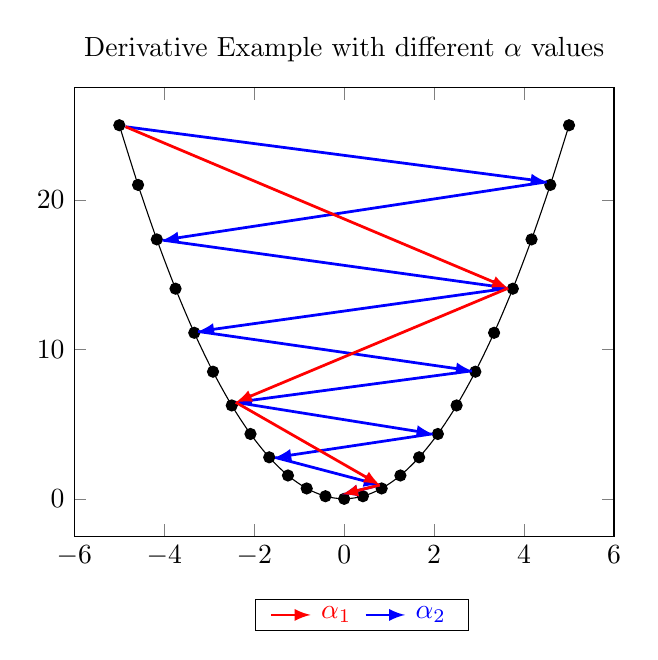
\begin{tikzpicture}
%\draw[step=.5, gray!40, very thin] (0,0) grid (7,5.5);
\begin{axis}[
% Show (automatically) computed limits:
title={
	Derivative Example with different $\alpha$ values},]
\addplot[mark=*,black,smooth] {x^2};
%\addlegendentry{$f(x)=x^2$};
%\addlegendimage{only marks,mark=*};
%\addlegendimage{only marks,mark=diamond*};
\end{axis}

\draw[arrows=-latex,line width=1pt,blue] (.65,5.2) -- (6,4.5);
\draw[arrows=-latex,line width=1pt,blue] (6,4.5) -- (1.12,3.76);
\draw[arrows=-latex,line width=1pt,blue] (1.12,3.76) -- (5.51,3.15);
\draw[arrows=-latex,line width=1pt,blue] (5.51,3.15)--(1.57,2.6);
\draw[arrows=-latex,line width=1pt,blue] (1.57,2.6)--(5.05,2.1);
\draw[arrows=-latex,line width=1pt,blue] (5.05,2.1)--(2.05,1.7);
\draw[arrows=-latex,line width=1pt,blue] (2.05,1.7) -- (4.55,1.3) ;
\draw[arrows=-latex,line width=1pt,blue]  (4.55,1.3) --(2.55,1);
\draw[arrows=-latex,line width=1pt,blue]  (2.55,1)--(3.88,.65);
\draw[arrows=-latex,line width=1pt,blue]  (3.88,.65)--(3.4,.53);

\draw[arrows=-latex,line width=1pt,red] (.65,5.2) -- (5.51,3.15);
\draw[arrows=-latex,line width=1pt,red] (5.51,3.15)--(2.05,1.7);
\draw[arrows=-latex,line width=1pt,red]  (2.05,1.7) --(3.88,.65);
\draw[arrows=-latex,line width=1pt,red]  (3.88,.65)--(3.4,.53);
\draw[arrows=-latex,line width=1pt,red]  (2.5,-1)-- (3,-1) node [right] {$\alpha_1$};
\draw[arrows=-latex,line width=1pt,blue]  (3.7,-1)-- (4.2,-1) node [right] {$\alpha_2$};
\draw  (2.3, -1.2) rectangle (5, -0.8);


\end{tikzpicture}
